\documentclass[tikz,border=10pt]{standalone}
\usepackage{tikz}
\usetikzlibrary{shapes.misc,shapes.geometric, arrows.meta, positioning, calc}

% Define styles for the nodes
\tikzset{
    ellipse box/.style={ellipse, draw, minimum width=1.5cm, minimum height=0.75cm, inner sep=0pt},
    rounded rect/.style={rounded rectangle, draw, minimum width=1.5cm, minimum height=0.75cm, inner sep=0pt},
    node/.style={font=\sffamily, fontsize=10pt}
}

% Define the main flow direction
\tikzset{
    edge/.style={-Stealth, thick},
    main flow/.style={->, >=Stealth, thick, shorten >=2pt, shorten <=2pt}
}

\colorlet{darkgreen}{green!60!black}
\begin{document}
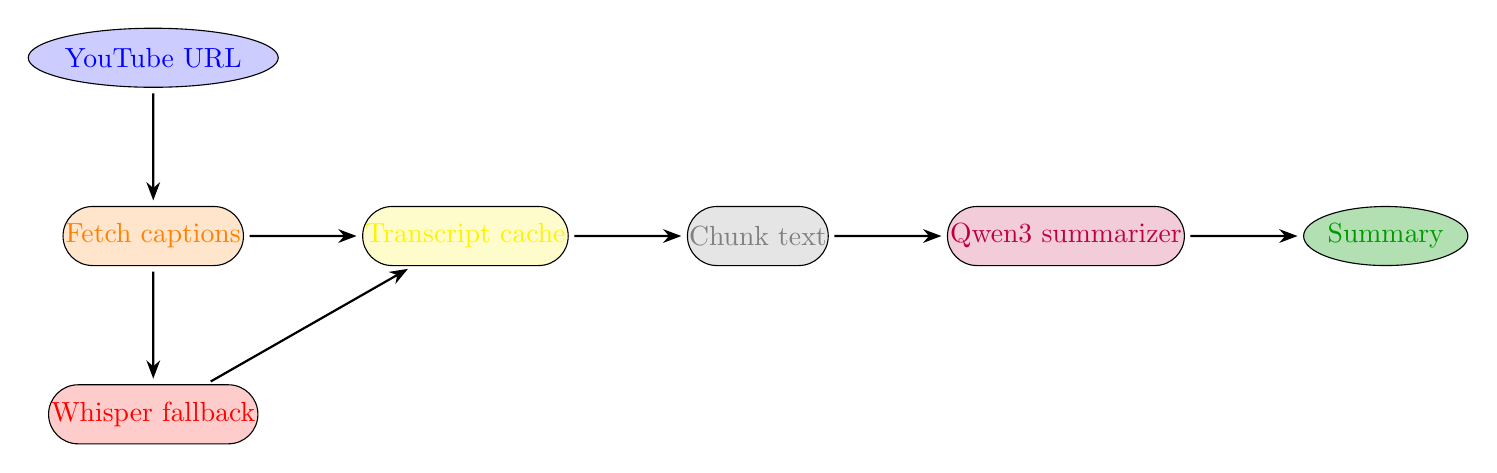
\begin{tikzpicture}[
    node distance=1.5cm and 1.5cm,
    start node/.style={ellipse box, fill=blue!20, text=blue},
    end node/.style={ellipse box, fill=green!20, text=green},
    fetch node/.style={rounded rect, fill=orange!20, text=orange},
    whisper node/.style={rounded rect, fill=red!20, text=red},
    cache node/.style={rounded rect, fill=yellow!20, text=yellow},
    chunk node/.style={rounded rect, fill=gray!20, text=gray},
    qwen node/.style={rounded rect, fill=purple!20, text=purple},
    summary node/.style={ellipse box, fill=darkgreen!30, text=darkgreen}
]

% --- Layout ---
% Start Node: YouTube URL
\node[start node] (url) {YouTube URL};

% Main Flow (Left to Right)
% Fetch captions
\node[fetch node, below=of url] (fetch) {Fetch captions};

% Whisper fallback (placed below Fetch captions as requested)
\node[whisper node, below=of fetch] (whisper) {Whisper fallback};

% Transcript cache (connected to both Fetch and Whisper)
\node[cache node, right=of fetch] (cache) {Transcript cache};

% Chunk text
\node[chunk node, right=of cache] (chunk) {Chunk text};

% Qwen3 summarizer
\node[qwen node, right=of chunk] (qwen) {Qwen3 summarizer};

% Output Node: Summary
\node[summary node, right=of qwen] (summary) {Summary};

% --- Edges ---
% 1. YouTube URL -> Fetch captions
\draw[main flow] (url) -- (fetch);

% 2. Fetch captions -> Transcript cache
\draw[main flow] (fetch) -- (cache);

% 3. Fetch captions -> Whisper fallback (labelled 'no captions')
\draw[main flow, edge label={no captions}] (fetch) -- (whisper);

% 4. Whisper fallback -> Transcript cache
\draw[main flow] (whisper) -- (cache);

% 5. Transcript cache -> Chunk text
\draw[main flow] (cache) -- (chunk);

% 6. Chunk text -> Qwen3 summarizer
\draw[main flow] (chunk) -- (qwen);

% 7. Qwen3 summarizer -> Summary
\draw[main flow] (qwen) -- (summary);

\end{tikzpicture}
\end{document}
